\documentclass[a4paper, 11pt, english]{article}
%
% Importering av pakker
%
\usepackage[utf8]{inputenc}
\usepackage[T1]{fontenc, url}
\usepackage[english]{babel}
\usepackage{textcomp}
\usepackage{amsmath, amssymb}
\usepackage{amsbsy, amsfonts}
\usepackage{graphicx, color}
\usepackage{parskip} % Space between paragraphs instead of indented text.
\usepackage{fancyhdr}
\usepackage{lastpage}
\usepackage{a4wide} % Smaller margins.
\usepackage{booktabs} % Functionality for tables.
\usepackage{lipsum} % Placeholder text
\usepackage{lmodern}
%
% Fancy captions
%
\usepackage[small,bf]{caption}
\usepackage{hyperref}
\usepackage{fancyhdr}
%
% Algorithms
%
\usepackage{algpseudocode}
\usepackage{algorithm}
%
% Subfigure functionality
%
\usepackage{caption}
\usepackage{subcaption}
%
% Parametere for inkludering av kode fra fil
%
\usepackage{listings}
%\lstset{language=python}
%\lstset{basicstyle=\ttfamily\small}
%\lstset{frame=single}
%\lstset{keywordstyle=\color{red}\bfseries}
%\lstset{commentstyle=\itshape\color{blue}}
\lstset{showspaces=false}
\lstset{showstringspaces=false}
\lstset{showtabs=false}
\lstset{breaklines}
\lstset{tabsize=4}
%
% Cool code listing
%
\lstdefinestyle{custompython}{
  belowcaptionskip=0.2\baselineskip,
  breaklines=true,
  frame=L,
  xleftmargin=\parindent,
  language=python,
  showstringspaces=false,
  basicstyle=\footnotesize\ttfamily,
  keywordstyle=\bfseries\color{red}\bfseries,
  commentstyle=\itshape\color{blue},
  identifierstyle=\color{black},
  stringstyle=\color{magenta},
}
\lstdefinestyle{customasm}{
  belowcaptionskip=1\baselineskip,
  frame=L,
  xleftmargin=\parindent,
  language=python,
  basicstyle=\footnotesize\ttfamily,
  commentstyle=\itshape\color{blue},
}
\lstset{escapechar=@,style=custompython}
%
% Pseudokode
%
\usepackage{xcolor}
\usepackage{listings}
\usepackage{caption}
\DeclareCaptionFont{white}{\color{white}}
\DeclareCaptionFormat{listing}{%
  \parbox{\textwidth}{\colorbox{gray}{\parbox{\textwidth}{#1#2#3}}\vskip-4pt}}
\captionsetup[lstlisting]{format=listing,labelfont=white,textfont=white}
\lstset{frame=lrb,xleftmargin=\fboxsep,xrightmargin=-\fboxsep}
%
% Definering av egne kommandoer og miljøer
%
\newcommand{\dd}[1]{\ \mathrm{d}#1} %
\newcommand{\D}[1]{\mathrm{d}#1}
\newcommand{\f}[2]{\frac{#1}{#2}}
\newcommand{\beq}{\begin{equation*}}
\newcommand{\eeq}{\end{equation*}}

\newcommand{\refeq}[1]{(\textcolor{red}{\ref{eq:#1}})} % Red color when referencing equations.
\newcommand{\refig}[1]{\textcolor{blue}{\ref{fig:#1}}} % Blue color when referencing figures.
\newcommand{\reflst}[1]{(\textcolor{red}{\ref{lst:#1}})}
\newcommand{\reftab}[1]{\textcolor{blue}{\ref{tab:#1}}} % Blue color when referencing tables.

\newcommand{\HRule}{\rule{\linewidth}{0.5mm}}

\newcommand{\course}{AST3310 - Astrophysical plasma and stellar interiors}
\newcommand{\handIn}{Project 2}
\newcommand{\projectTitle}{Numerical modeling of stellar interior}

%
% Page formatting
%
%\pagestyle{fancy}
%\lhead{Vedad Hodzic}
%\rhead{}
%\cfoot{ \thepage\ of \pageref{LastPage} }
%
% Navn og tittel
%

\author{Vedad Hodzic}

\begin{document}

\begin{titlepage}
    \thispagestyle{empty}
    % Explanation of \\[]-syntax: 
% In the square brackets you can define a certain vertical space
% which is inserted in the text. Convenient for fancy formatting.

\begin{center}
    \LARGE University of Oslo\\[1.5cm]
	\Large \course \\ 
	\Large \handIn \\ [0.5cm]
    \HRule \\[0.4cm]

    % Title of project
    { \huge \bfseries \projectTitle \\[0.4cm] }

    \HRule \\[1.5cm]

    % Spaces between lines are there for line breaks

	\large Vedad Hodzic

    \vfill

    {\large \today}
\end{center}

\end{titlepage}

\begin{abstract}
	I here discuss the physical properties of stellar interiors based on models and
	simplifications addressed in ~\cite{stix} and ~\cite{gudiksen}. Numerical calculations
	are used to solve the governing equations of the interior of stars. Models for
	convective, as well as radiative, energy transfer are included and discussed. For a
	given set of initial conditions, one should expect the luminosity, position and mass
	to end at zero value simultaneously as the core is reached. The best model to achieve
	this within the limit of 10\% of initial value has initial physical properties
	$L_0 = L_{\odot}$, $M_0 =
	1.5M_{\odot}$, $R_0 = 9R_{\odot}$, $T_0 = 5770$ K, $\rho_0 = 4.0 \times 10^{-7}$ g
	$\mathrm{cm}^{-3}$. To this end, I apply an adaptive step method.
	It is found that the results heavily depend on initial properties,
	as well as the constraints on the mass step $\D{m}$.
\end{abstract}

\section{Introduction}

There are four differential equations that govern the internal structure of stellar
objects in our
model. I apply here numerical methods such as the Euler integration scheme to solve these
equations. This involves solving equations for nuclear fusion as well as ordinary
differential equations. We include radiation and convection models, and look at how 
the interior of solar-like stars changes based on
different initial
parameters. I try to seek out a set of parameters that leads to the case where mass,
radius and luminosity reach zero value simultaneously. 

\section{Theory}
\subsection{General background}

The equations that regulate the physical properties of stellar interiors are
expressed as
%%%
\begin{align}
	\frac{\partial r}{\partial m} &= \frac{1}{4\pi r^2 \rho} \label{eq:drdm} \\
	\frac{\partial P}{\partial m} &= -\frac{Gm}{4\pi r^4} \label{eq:dPdm} \\
	\frac{\partial L}{\partial m} &= \varepsilon \label{eq:dLdm} \\
	\frac{\partial T}{\partial m} &= -\frac{3 \kappa L}{256 \pi^2 \sigma r^4 T^3}. 
	\label{eq:dTdm} 
\end{align}
%%%
The parameter $\varepsilon$ in Eq.~\refeq{dLdm} is the total energy generation per unit mass.
It is found by looking at the energy generation from nuclear reactions. It depends on the
abundancy of different elements, temperature and density. The variable $\kappa$ is the
opacity, which is an average of frequency of photons.
The pressure in Eq.~\refeq{dPdm} is a sum of the gas pressure $P_{\mathrm{G}}$,
and the radiative pressure $P_{\mathrm{R}}$. 
\begin{align}
	P &= P_{\mathrm{G}} + P_{\mathrm{R}} \nonumber \\
	P &= \frac{\rho}{\mu m_{\mathrm{u}}} kT + \frac{a}{3}T^4 \nonumber \\
	\Rightarrow \rho &= \frac{\mu m_{\mathrm{u}}}{kT} \left( P - \frac{a}{3}T^4 \right),
	\label{eq:density}
\end{align}
which yields the density derived from the equation of state. Here, $m_{\mathrm{u}}$ is the
atomic mass unit and $k$ is the Boltzmann
constant. The constant $a$ is defined as $a = 4\sigma / c$, where $\sigma$ is the
Stefan-Boltzmann constant, and $c$ is the speed of light. The average molecular weight
$\mu$ is found by
\begin{align}
	\mu = \frac{1}{m_{\mathrm{u}}}\frac{\rho}{n_{\mathrm{tot}}}.
	\label{eq:mu}
\end{align}
We can find the total particle density $n_{\mathrm{tot}}$ with
\begin{align*}
	n_{\mathrm{tot}} &= n_X + n_Y + n_Z + n_e \\
	&= \frac{X\rho}{m_{\mathrm{u}}} + \frac{Y\rho}{4m_{\mathrm{u}}} +
	 \left( \frac{X\rho}{m_{\mathrm{u}}} +
	 \frac{2Y\rho}{4m_{\mathrm{u}}}\right) + \sum\limits_i (n_{Z_i} + n_{e,Z_i})
%	\frac{Z\rho}{A_im_{\mathrm{u}}} + \frac{1}{2}A_i \frac{Z\rho}{2m_{\mathrm{u}}} \right),
\end{align*}
The sum is over the heavier metals present in the star. The number of atoms and electrons
for an element $i$ is
\begin{align*}
	n_{Z_i} = \frac{Z_i \rho}{m_{Z_i}} = \frac{Z_i \rho}{A_i m_{\mathrm{u}}} \\
	n_{e,Z_i} = \frac{1}{2}A_i \frac{Z_i \rho}{A_i m_{\mathrm{u}}},
\end{align*}
where $A_i$ is the mass number; the total number of particles in the element nuclei. For
the heavier elements to be fully ionised, we have assumed that these elements have released
half as many electrons as their atomic mass, $A_i$. We therefore assume that the nucleus is
half neutrons and half protons. The
number density of heavier metals is then
\begin{align*}
	\sum\limits_i (n_{Z_i} + n_{e,Z_i}) = \sum\limits_i \left(\frac{Z_i \rho}{A_i
		m_{\mathrm{u}}} + \frac{1}{2}A_i \frac{Z_i \rho}{A_i m_{\mathrm{u}}} \right) \approx
		\frac{Z \rho}{2 m_{\mathrm{u}}},
\end{align*}
where we assumed that the first term in the sum is negligible compared to the second term,
because $A$ can be rather large. We then have for the total number density
\begin{align*}
	n_{\mathrm{tot}} = \frac{2 X \rho}{m_{\mathrm{u}}} + \frac{3 Y \rho}{4
		m_{\mathrm{u}}} + \frac{Z \rho}{2 m_{\mathrm{u}}},
\end{align*}
and the average molecular weight is then
\begin{align*}
	\mu &= \frac{\rho m_{\mathrm{u}}}{\rho m_{\mathrm{u}}} \left( \frac{1}{2X +
		\frac{3}{4}Y + \frac{1}{2}Z} \right) \\
		&= \frac{1}{2X +\frac{3}{4}Y + \frac{1}{2}Z},
\end{align*}
assuming all elements are fully ionised.

The total energy generation per unit mass $\varepsilon$, is found by
\begin{align}
	\varepsilon = \sum Q'_{ik} r_{ik},
	\label{eq:epsilon}
\end{align}
where $i,k$ represents two elements, $Q'_{ik}$ is the energy released from the fusion of
two elements, $r_{ik}$ is the reaction rates per unit mass for two elements. The energies
$Q'_{ik}$ from the pp chains are listed in ~\cite[p.~39, Table~2.1]{stix}. The reaction
rates per unit mass is defined by
\begin{align}
	r_{ik} = \frac{n_i n_k}{\rho(1 + \delta_{ik})} \lambda_{ik},
	\label{eq:r}
\end{align}
where $n_i,n_k$ is the number density for an element, $\delta_{ik}$ is the Kronecker delta and
$\lambda_{ik}$ is the reaction rate of a fusion. The number density of an element is
easily defined as
\begin{align}
	n_i = \frac{\rho \chi_i}{A_im_{\mathrm{u}}},
	\label{eq:n}
\end{align}
where $\chi$ is the mass fraction of an element, and $A$ is the mass number of the
element. We denote $X, Y, Z$ to be the mass fractions of hydrogen, helium and heavier
metals, respectively. Finally, the reaction rates $\lambda_{ik}$ for two elements
$i,k$ can be found in ~\cite[p.~46, Table~2.3]{stix}.

\subsection{Convection}
In this model, we consider two means of energy transport in the star: radiation and
convection. Convection is the mass movement of plasma where warm plasma ascends 
and cooled plasma descends through the star.  A parcel of gas that is adiabatically
lifted from its
equilibrium position can either be heavier or lighter than its new environment. If
lighter, it will continue to rise, meaning the original equilibrium was unstable. If it is
heavier, it will return to its original position, meaning it was in a stable equilibrium.
The onset of convection is determined from
the Schwarzschild criterion, which describes the properties for stability and instability.
The criterion is often written as
\begin{align*}
	\nabla > \nabla_{\mathrm{ad}},
\end{align*}
where 
\begin{align}
	\nabla = \frac{\partial \ln T}{\partial \ln P},
	\label{eq:nabla_def}
\end{align}
is the temperature gradient, and $\nabla_{\mathrm{ad}}$ is its adabatic value. 
Eq.~\refeq{dTdm} only holds for radiative energy transport, which means we
need a way of finding $\partial T$, the change in temperature over an infinitessimal step
in a convective layer.
From Eq.~\refeq{nabla_def} we find
\begin{align}
	\nabla &= \frac{\partial \ln T}{\partial \ln P} \nonumber \\
	&= \frac{P}{T}\frac{\partial T}{\partial P} \nonumber \\
	&= \frac{P}{T}\frac{\partial T}{\partial m} \frac{\partial m}{\partial P} \nonumber \\
	\Rightarrow \partial T &= \frac{T}{P} \partial P \nabla, \label{eq:dt_conv}
\end{align}
which gives us the change in temperature in a convectively unstable layer.

We now need to find an expression for the true temperature gradient $\nabla$.
%It is found by 
We know that
the total energy flux is
\begin{align*}
	F_{\mathrm{R}} + F_{\mathrm{C}} &= \frac{L}{4\pi r^2} \\
	&= \frac{4 a c G T^4 m}{3 \kappa Pr^2}\nabla_{\mathrm{rad}},
\end{align*}
where
\begin{align*}
	F_{\mathrm{R}} &= \frac{4acGT^4m}{3 \kappa P r^2} \nabla \\
	F_{\mathrm{C}} &= \rho c_P T \sqrt{g \delta} H_P^{-3/2} \left(
	\frac{l_{\mathrm{m}}}{2} \right)^2 (\nabla - \nabla^*)^{3/2}.
\end{align*}
We use these to get an expression between $\nabla, \nabla_{\mathrm{rad}}$ and $\nabla^*$.
\begin{align*}
	F &= F_{\mathrm{R}} + F_{\mathrm{C}} \\
	\Rightarrow \frac{4 a c G T^4 m}{3 \kappa Pr^2}\nabla_{\mathrm{rad}} &=
	\frac{4acGT^4m}{3 \kappa P r^2} \nabla + \rho c_P T \sqrt{g \delta}
	H_P^{-3/2} \left(
	\frac{l_{\mathrm{m}}}{2} \right)^2 (\nabla - \nabla^*)^{3/2}\\
	\Rightarrow (\nabla - \nabla^*)^{3/2} &= \frac{\rho H_P G m}{Pr^2
	l_{\mathrm{m}}} \frac{16acT^3}{3 \kappa \rho^2 c_P}
	\sqrt{\frac{H_P}{g \delta}}(\nabla_{\mathrm{rad} - \nabla}).
\end{align*}
We insert $a = 4 \sigma / c$ and note that
\begin{align*}
	U &= \frac{64 \sigma T^3}{3 \kappa \rho^2 c_P} \sqrt{\frac{H_P}{g \delta}} \\
	H_P &= \frac{Pr^2}{G \rho m},
\end{align*}
and then have
\begin{align*}
	(\nabla - \nabla^*)^{3/2} &= \frac{U}{l_{\mathrm{m}}^2}(\nabla_{\mathrm{rad}} -
	\nabla).
\end{align*}
Furthermore, we have 
\begin{align*}
	(\nabla^* - \nabla_{\mathrm{ad}}) &= (\nabla - \nabla_{\mathrm{ad}}) - (\nabla -
	\nabla^*) \\
	\Rightarrow U\left( \frac{S}{d Q l_{\mathrm{m}}} \right) (\nabla - \nabla^*)^{1/2} &=
	(\nabla - \nabla_{\mathrm{ad}}) - (\nabla - \nabla^*),
\end{align*}
which can be rewritten to a second order equation for $(\nabla - \nabla^*)^{1/2}$. We
rename $(\nabla - \nabla^*)^{1/2} = \xi$ and find
\begin{align}
	0 &= \xi^2 + K\xi - (\nabla - \nabla_{\mathrm{ad}}) \nonumber \\
	\Rightarrow \nabla &= \xi^2 + K\xi + \nabla_{\mathrm{ad}} \label{eq:nabla_real},
\end{align}
where $K = 4R$, $R = U/l_{\mathrm{m}}^2$. We now have an expression for the true
temperature gradient, but we need $\xi$. It can be found that
\begin{align*}
	\xi^3 + R\xi^2 + RK\xi - (\nabla_{\mathrm{rad}} - \nabla_{\mathrm{ad}}) = 0.
\end{align*}
This equation yields three roots. Two are complex conjugates and one is real. We can
easily solve this equation numerically to find the real root, and insert it in
Eq.~\refeq{nabla_real} to find the temperature gradient. This can then be used to
calculate $\partial T$ in Eq.~\refeq{dt_conv}.

\section{Algorithm}
\subsection{Simplifications}

In order to make a simple model I needed some simplifications. A list of
assumptions and simplifications follows.
\begin{itemize}
	\item[\textbullet] There is no change in the composition of elements as a function of
		radius. 
	\item[\textbullet] I assume there is no change in the density of deuterium, so that
		the rate of destruction of deuterium is the same as the production, and that any
		reaction involving deuterium happens instantaneous.
	\item[\textbullet] All nuclear energy comes from the three PP-chains. I have not
		included the CNO cycle.
	\item[\textbullet] I assume all elements to be fully inonised.
\end{itemize}

\subsection{Units}

Given that $\kappa$ is in units of $\left[\mathrm{cm}^2  \ \mathrm{g}^{-1}\right]$ and
$\lambda$ in units of $\left[\mathrm{cm}^3 \ \mathrm{s}^-1 \right]$,
I chose to adapt the CGS unit system (centimetre-gram-second). Table \reftab{units} shows
an overview of the differences.
\begin{table}
	\centering
	\begin{tabular*}{\textwidth}{p{0.25\textwidth}@{\extracolsep{\fill}}p{0.15\textwidth}p{0.15\textwidth}p{0.15\textwidth}p{0.15\textwidth}}
		\toprule
		\toprule
		& \multicolumn{4}{c}{Unit system} \\
		\cmidrule{2-5}
		& \multicolumn{2}{c}{CGS} & \multicolumn{2}{c}{SI} \\
		\cmidrule{2-3}
		\cmidrule{4-5}
		Physical property & Unit name & Unit abbr. & Unit name & Unit abbr. \\
		\midrule
		Length & centimetre & cm & metre & m \\
		Weight & gram & g & kilogram & kg \\
		Time & second & s & second & s \\
		Temperature & kelvin & K & kelvin & K \\
		Energy & erg & erg & joule & J \\
		Pressure & barye & Ba & pascal & Pa \\
		\bottomrule
		\bottomrule
	\end{tabular*}
	\caption{Overview of the difference between CGS units and SI units.}
	\label{tab:units} 
\end{table}


\subsection{Structure}

We see from Eq.~\refeq{dTdm} that $\partial T / \partial m$ depends on the opacity,
$\kappa$. A table of opacities that correspond to different values of temperature and
density has been provided. I wrote a function that reads the file and stores values of
$T$, $R$ and $\kappa$ in separate arrays. Here, $R = R(T, \rho) = \rho / T_6$. The
function compares the table temperature with the
actual temperature, and the same with the variable $R$. It returns the $\kappa$ with
table values of $T$ and $R$ that most closely resembles the present values.

Next, I wrote a function that calculates the energy generation per mass unit from nuclear
reactions. This means entering the energy releases $Q'_{ik}$ from ~\cite[p.~39,
Table~2.1]{stix}, the reaction rates $\lambda_{ik}$ from ~\cite[p.~46,
Table~2.3]{stix} and finding the number densities $n$ for all particles that are involved
in a nuclear reaction. Given the mass fractions $X,Y,Z$ and sub-fractions of these
for different elements, I was able to calculate the energy generation per mass by using
Eqs.~\refeq{epsilon}, \refeq{r} and \refeq{n}. The function also returns the distribution
of energy generation between the three pp chains.

I have a function that calculates the density at present time, given the temperature
$T$ and total pressure $P$. This is found from the equation of state, as given in Eq.
\refeq{density}. This required me to calculate the average molecular weight $\mu$,
shown in Eq.~\refeq{mu}. Another function calculates the pressure at any layer, which is
also derived from the equation of state.

Three functions calculate the convective, radiative and total flux. These are useful to
see the fraction of energy transported by convection and radiation.

Further, I have four functions that return the right-hand side in Eqs.~\refeq{drdm},
\refeq{dPdm}, \refeq{dLdm} and \refeq{dTdm}. These are called upon in another function
that integrates all the equations.

Lastly, the function that integrates the equations contains a test for convective
stability, calculating $\dd{T}$ based on convection if the layer is convective unstable.
This is done by finding the one real root of a cubic polynomial numerically, then using
the solution in finding the true temperature gradient, including convection, of the star.
This function also implements an adaptive step method. See
Section~(\ref{sec:adaptive_mass_step}) for details.


\subsection{The Euler integration scheme}

For simplicity, I have chosen the Euler integration scheme to integrate the differential
equations. Listing \reflst{integration} shows how it is carried out.
\belowcaptionskip=-10pt
\begin{lstlisting}[label=lst:integration,caption=Euler integration loop]	
while m > 0:
	r_new = r_old + (dr/dm) * dm
	P_new = P_old + (dP/dm) * dm
	L_new = L_old + (dL/dm) * dm
	T_new = T_old + (dT/dm) * dm
	m_new = m_old + dm
\end{lstlisting}
The Euler method advances one step by adding the previous step value to the current value
of the right-hand side of the differential equations, multiplied by the mass step.
Unfortunately, the scheme carries a local truncation error proportional to the step size
squared, and a global truncation error that is proportional to the step size.

\subsection{Adaptive mass step}
\label{sec:adaptive_mass_step}
To avoid sudden and large changes in $r,T,L,P$, I implement an adaptive step method that
calculates the mass step $\dd{m}$ by applying constraints on how much the physical
parameters are allowed to increase or decrease from one step to another. By applying a
constraint on the relative change in radius, i.e. $\dd{r}/r \leq 0.2$, we are guaranteed
that the relative change in radius will not exceed 20 \%. The corresponding mass step can
be easily found from
\begin{align*}
	\frac{\D{r}}{r} &\leq 0.2 \\
	\frac{\D{r}}{r}\frac{\D{m}}{\D{m}} &\leq 0.2 \\
	\D{m} \frac{\D{r}}{\D{m}} \frac{1}{r} &\leq 0.2 \\
	\D{m} &\leq 0.2 \frac{r}{\left( \frac{\D{r}}{\mathrm{d}m} \right)},
\end{align*}
and when integrating inwards, $\mathrm{d}m < 0$, so that
\begin{align*}
	\mathrm{d}m \leq -0.2 \left| \frac{r}{\left( \frac{\D{r}}{\mathrm{d}m} \right)}\right|.
\end{align*}
The same calculation can be done for the other physical parameters with the same
constraint, or another. By finding the $\D{m}$ that is smallest in absolute value of
$r/(\D{r}/\D{m})$, $T/(\D{T}/\D{m})$, $L/(\D{L}/\D{m})$, $P/(\D{P}/\D{m})$,
with each their own constraint, we are guaranteed
that they will all be fulfilled. I apply another constraint on $\D{m}$ itself, so that it
cannot increase or decrease more than a certain percentage of its previous value.

\subsection{Initial conditions}
Finally, we need a set of initial conditions to initiate the calculations. These are shown
in Table \reftab{initcond} expressed in the CGS unit system (see Table \reftab{units}).
\begin{table}
	\centering
	\begin{tabular*}{\textwidth}{p{2cm}@{\extracolsep{\fill}}p{3.5cm}p{2cm}p{2cm}}
		\toprule
		\toprule
		\multicolumn{2}{c}{Physical properties} & \multicolumn{2}{c}{Element abundancies}\\
		\cmidrule{1-2}
		\cmidrule{3-4}
		Parameter & Initial value & Element & Initial value \\
		\midrule
		$ L_0 $ & $ L_{\odot} $ & $X$ & 0.7 \\
		$ R_0 $ & $ R_{\odot}$ & $Y_3$ & $10^{-10}$ \\
		$ M_0 $ & $ M_{\odot}$ & $Y$ & 0.29 \\
		$\rho_0$ & $4.0 \times 10^{-7}$ g $\mathrm{cm}^{-3}$ & $Z$ & 0.01 \\
		$ T_0 $ & $5770$ K & $ Z_{^{7}{\mathrm{Li}}} $ & $10^{-12} $ \\
		$ P_0 $ & $3.1 \times 10^{5} $ Ba & $ Z_{^{7}{\mathrm{Be}}} $ & $10^{-12}$ \\
		\bottomrule
		\bottomrule
	\end{tabular*}
	\caption{Table that shows the initial physical parameters needed in order to initiate the
	calculations.}
	\label{tab:initcond}
\end{table}


\section{Results}
\subsection{Model with original initial conditions}
If we carry out the integration using the initial values as given in Table
\reftab{initcond}, we get the evolution for the physical parameters \(r,m,T,P\) as shown
in Fig.~\refig{init_results}. Fig.~\refig{luminosity_init} shows that the luminosity
reaches zero a little premature in relation to the position. This means that the
luminosity is the limiting parameter here, stopping the integration.
However, it shows what we expect of a luminosity graph as we integrate towards the center.
The mass plot is shown in Fig.~\refig{mass_init}. It falls short because of the
luminosity, but we see it lags considerably behind the position as well. The temperature
graph shows a larger increase towards the end which seems reasonable. It ends at
$T \approx 12$ MK, which is within reason at $r < 0.2R_{\odot}$. The pressure grows
incredibly fast towards the end, as the radiative pressure increases from the increase in
temperature.
\begin{figure}[htpb]
	\begin{subfigure}{0.49\textwidth}
		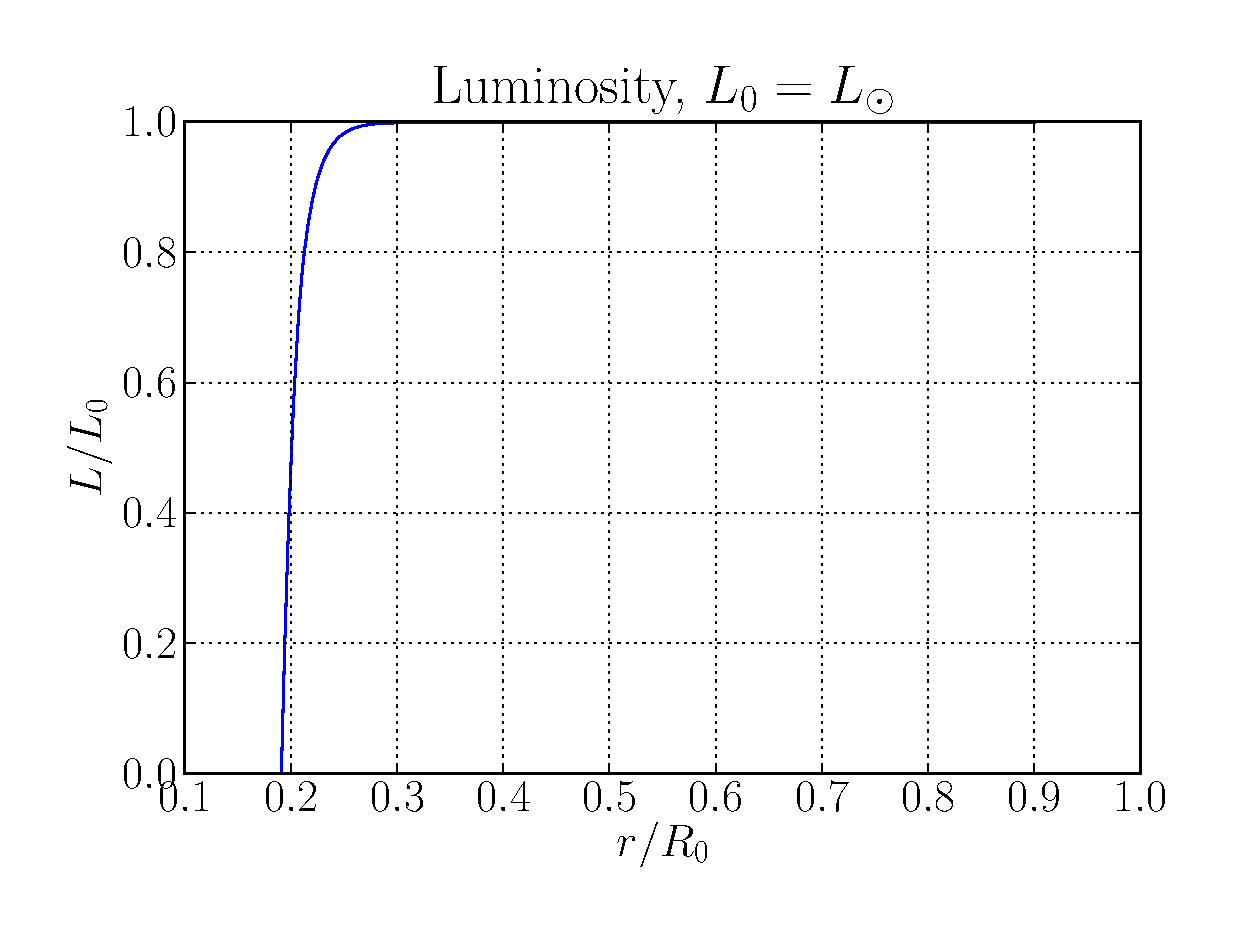
\includegraphics[width=\linewidth]{figures/luminosity_initial.eps}
		\caption{Luminosity}
		\label{fig:luminosity_init}
	\end{subfigure}\hfill
	\begin{subfigure}{0.49\textwidth}
		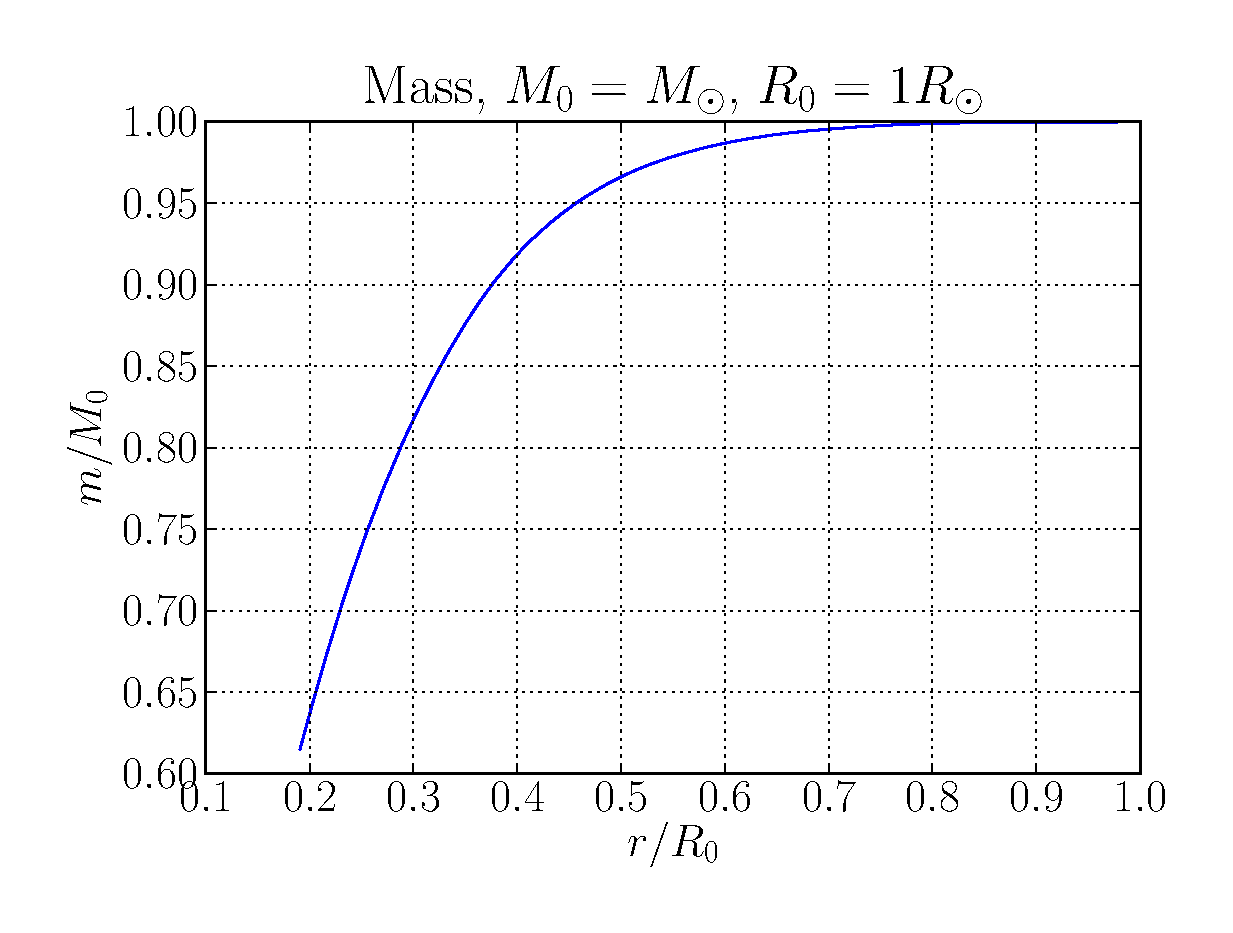
\includegraphics[width=\linewidth]{figures/mass_initial.eps}
		\caption{Mass}
		\label{fig:mass_init}
	\end{subfigure}\hfill
	\vspace{0.35cm}
	\begin{subfigure}{0.49\textwidth}
		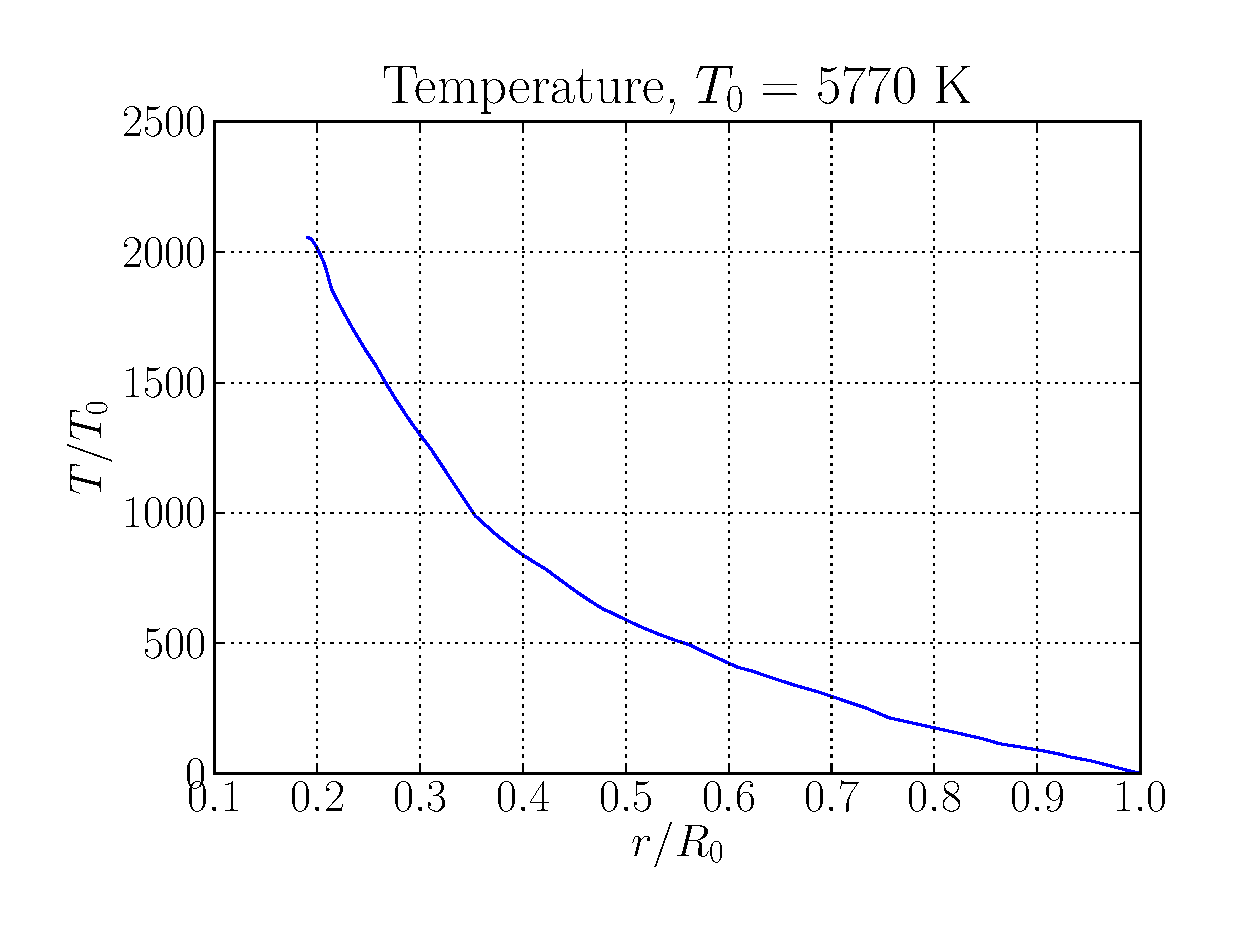
\includegraphics[width=\linewidth]{figures/temperature_initial.eps}
		\caption{Temperature}
		\label{fig:temperature_init}
	\end{subfigure}\hfill
	\begin{subfigure}{0.49\textwidth}
		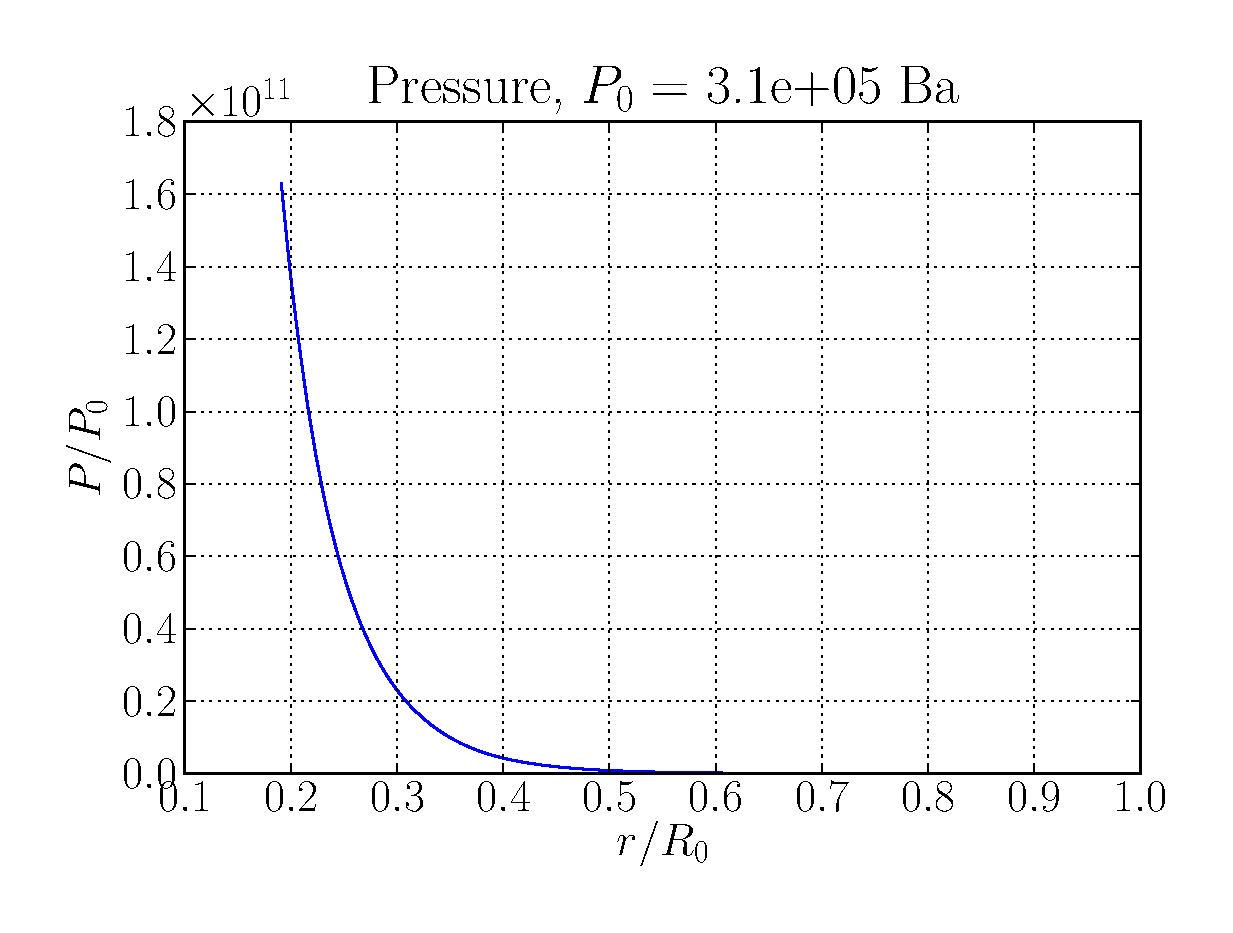
\includegraphics[width=\linewidth]{figures/pressure_initial.eps}
		\caption{Pressure}
		\label{fig:pressure_init}
	\end{subfigure}
	\vspace{0.2cm}
	\caption{The results from using initial conditions as described in
		Table~\reftab{initcond}.}
		\label{fig:init_results}
\end{figure}

\subsection{The best model}
The best parameters were found by trial and error. The result is shown in
Fig.~\refig{parameters_9Rsun}. We were able to integrate all the way to the core, ending
with mass $M_{\mathrm{end}} = 0.1M_{\odot}$. The temperature in the core is of the order $T \approx 18$
MK. which is slightly higher than the temperature in the core of the Sun. However, we 
are considering a star with a higher mass and larger radius, making the temperature
reasonable. The pressure has increased by a factor 100 billion in the core, relative to
the surface pressure. This seems
reasonable as the radiative pressure increases by temperature to the power of four, making
it within limits.

\begin{figure}[htpb]
	\begin{subfigure}{0.49\textwidth}
		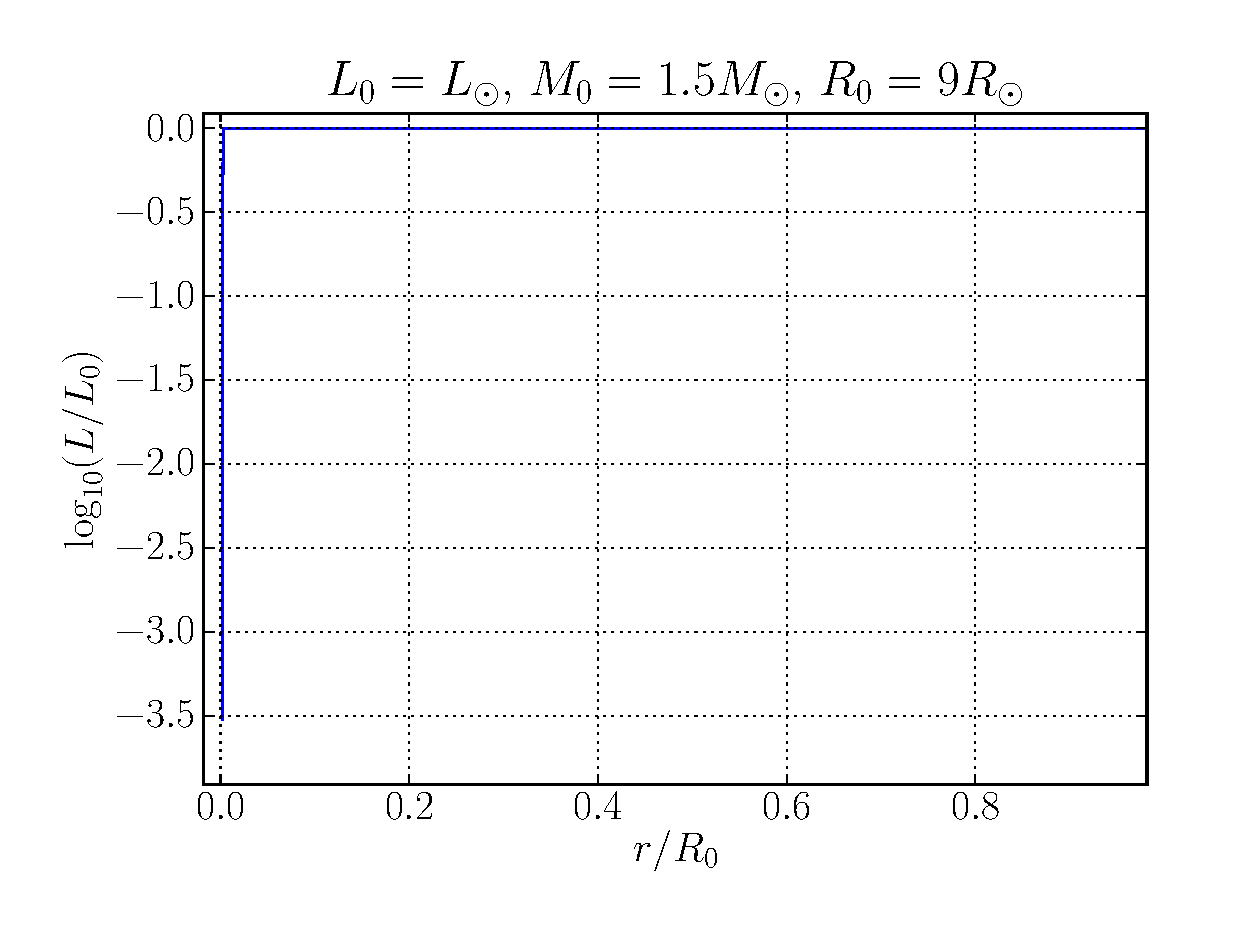
\includegraphics[width=\linewidth]{figures/luminosity_1-5Msun.eps}
		\caption{Luminosity}
		\label{fig:luminosity_9Rsun}
	\end{subfigure}\hfill
	\begin{subfigure}{0.49\textwidth}
		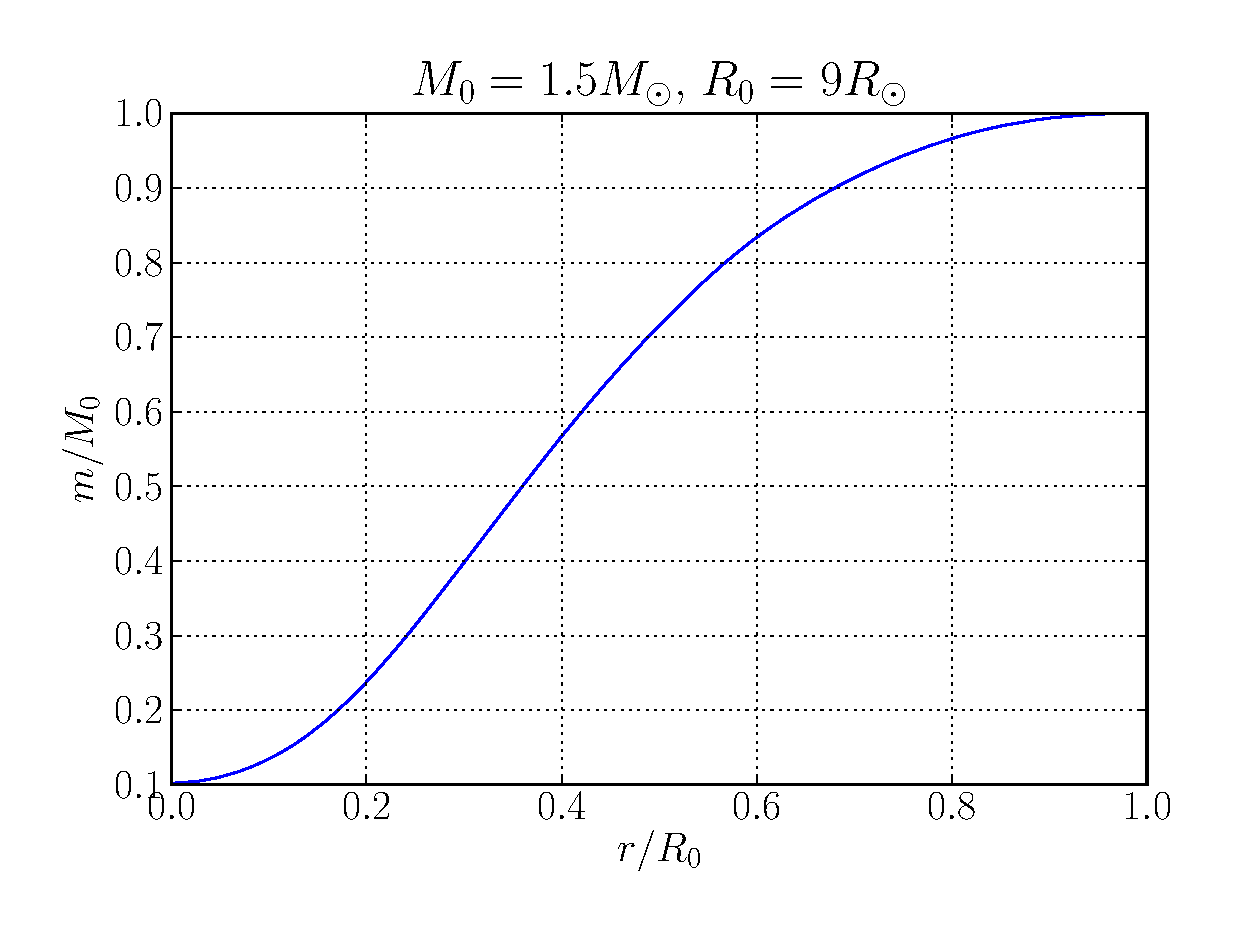
\includegraphics[width=\linewidth]{figures/mass_1-5Msun.eps}
		\caption{Mass}
		\label{fig:mass_9Rsun}
	\end{subfigure}\hfill
	\vspace{0.35cm}
	\begin{subfigure}{0.49\textwidth}
		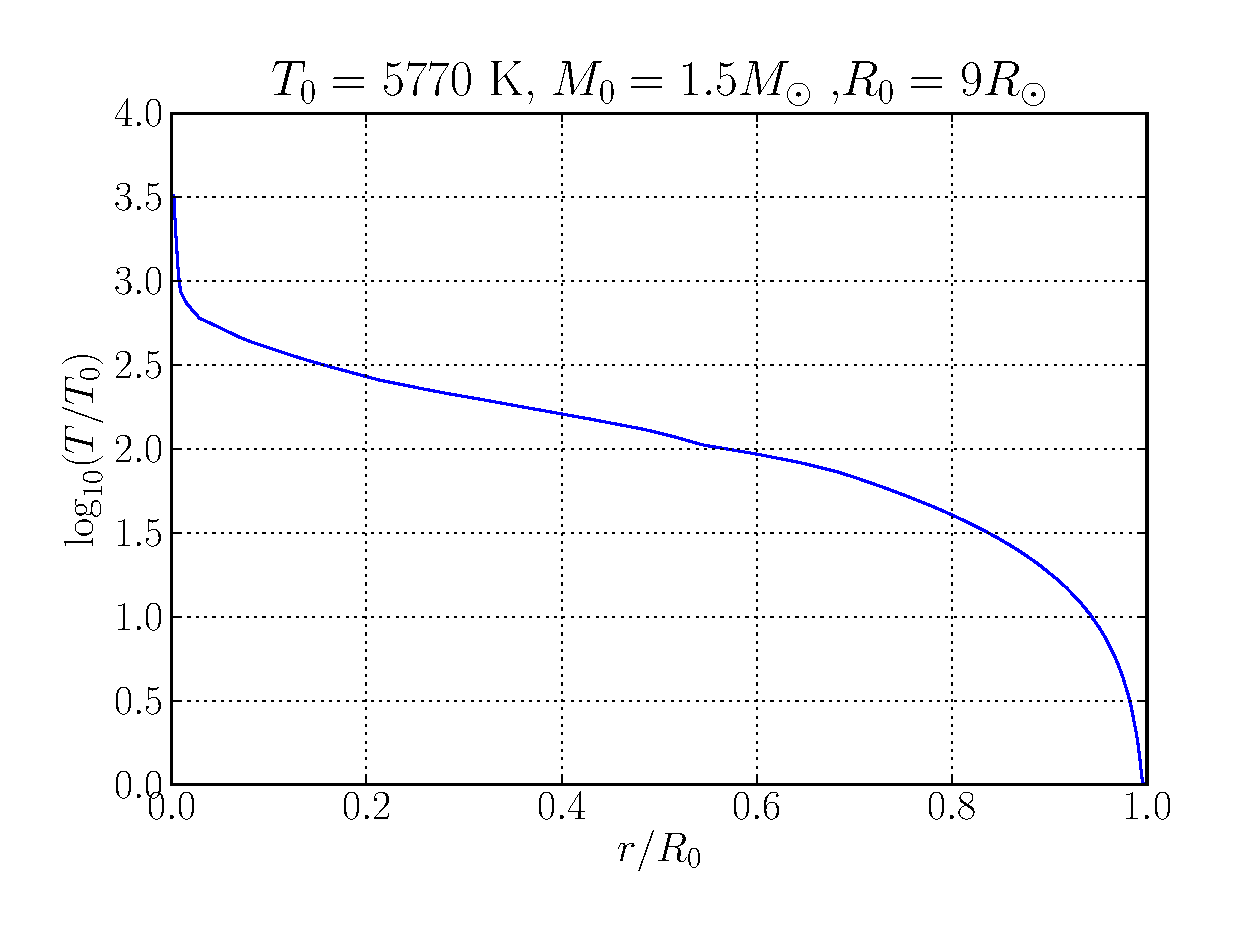
\includegraphics[width=\linewidth]{figures/temperature_1-5Msun.eps}
		\caption{Temperature}
		\label{fig:temperature_9Rsun}
	\end{subfigure}\hfill
	\begin{subfigure}{0.49\textwidth}
		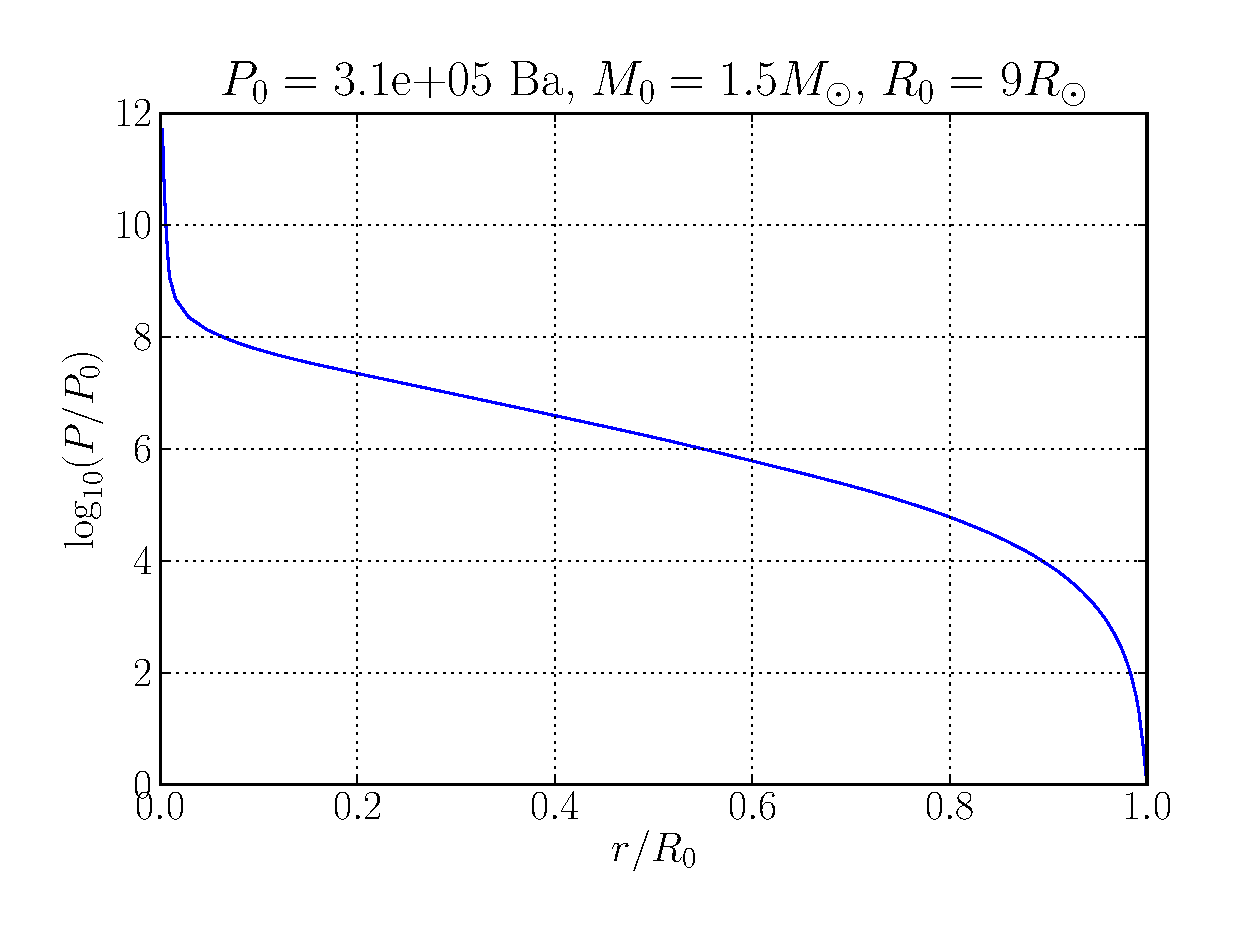
\includegraphics[width=\linewidth]{figures/pressure_1-5Msun.eps}
		\caption{Pressure}
		\label{fig:pressure_9Rsun}
	\end{subfigure}
	\vspace{0.2cm}
	\caption{The results from using the physical parameters giving the best model of a
		star. $M_0 = 1.5M_{\odot}$, $R0 = 9R_{\odot}$, $T0 = 5770$ K, $P0 = 3.1 \times
	10^5$ Ba.}
		\label{fig:parameters_9Rsun}
\end{figure}

%It is of interest to see the fraction of energy transported by convection and radiation.
%We find that Fig.~\refig{flux_distribution} shows the flux distribution. Convection only
%becomes dominant in the last $5$ \% of the outer layer, meaning we have a poor convection
%model for these initial conditions. The energy generation in Fig.~\refig{energy_gen_init}
%shows a sudden increase in nuclear reactions towards the end, which indeed makes sense.
%However, the distribution between the PP-chains relative to the total energy production
%seems odd, as $\varepsilon$ increases, but none of the energy generation from the PP-chains.
%\begin{figure}[htpb]
%	\begin{subfigure}{0.49\textwidth}
%		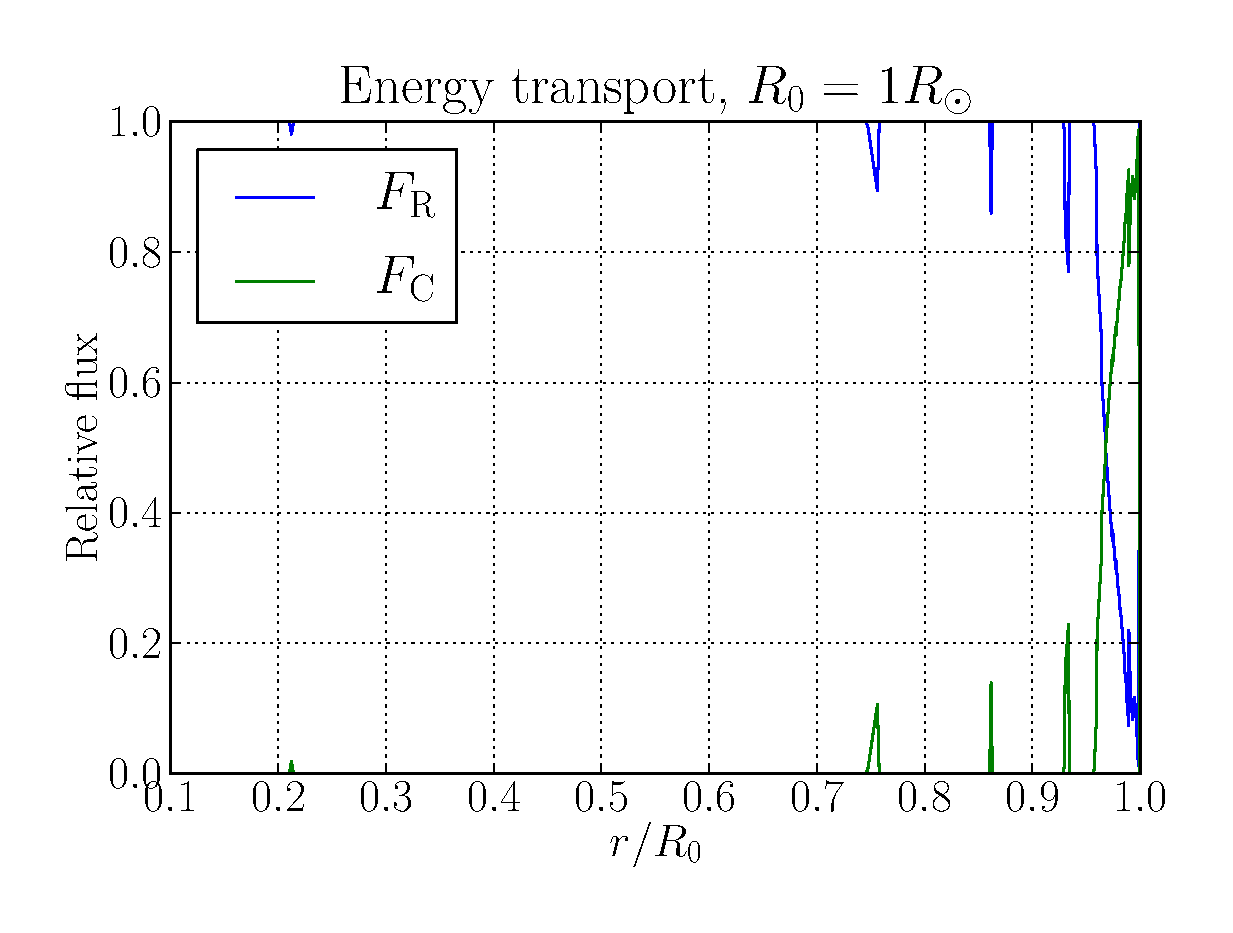
\includegraphics[width=\linewidth]{figures/flux_initial.eps}
%		\caption{Flux distribution}
%		\label{fig:flux_distribution}
%	\end{subfigure}\hfill
%	\begin{subfigure}{0.49\textwidth}
%		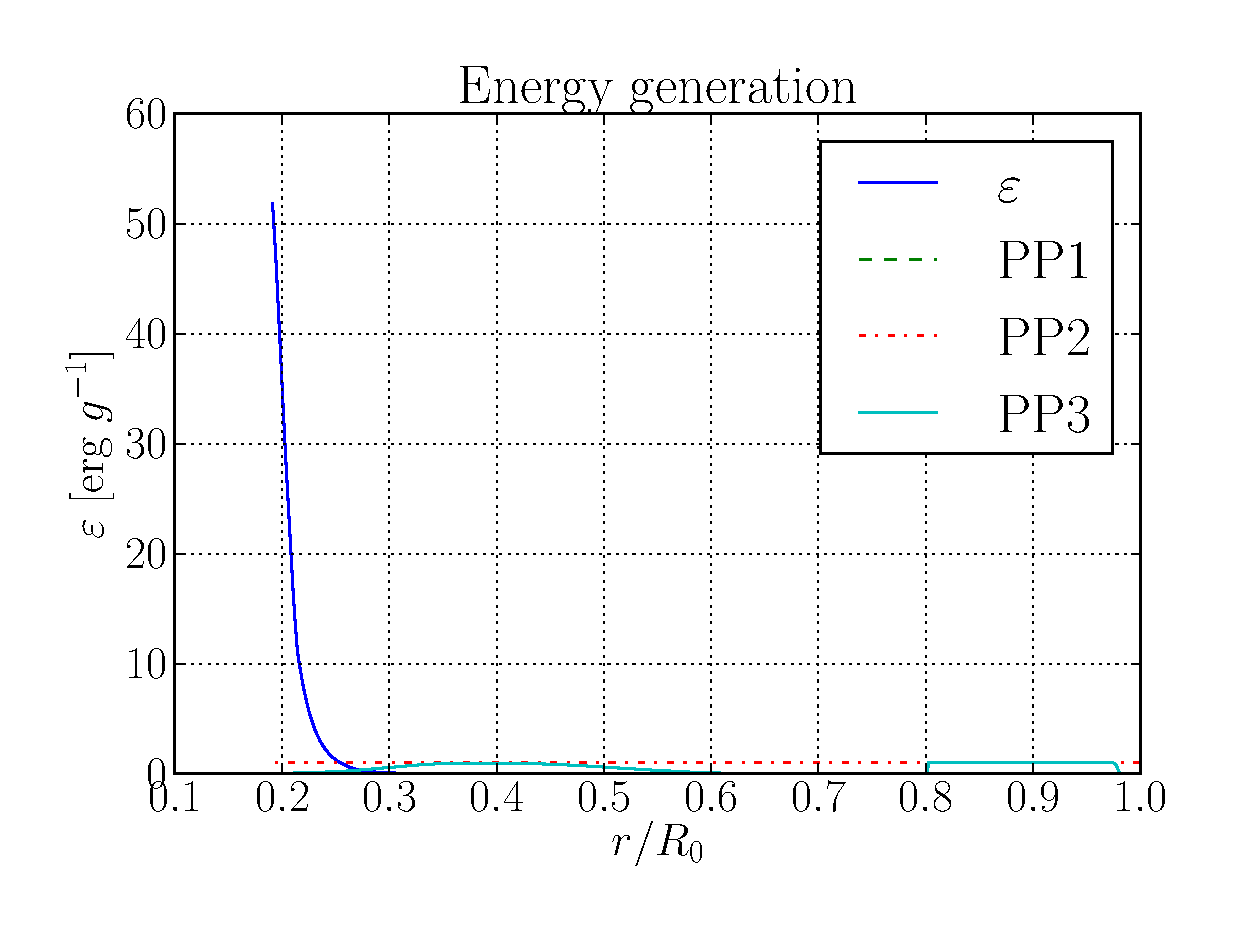
\includegraphics[width=\linewidth]{figures/energy_initial.eps}
%		\caption{Energy generation}
%		\label{fig:energy_gen_init}
%	\end{subfigure}
%	\caption{The fraction of energy transported by convection and radiation to the left,
%	and the distribution of energy generation amongst the PP-chains.}
%\end{figure}

\subsection{Changing the initial radius}
\subsubsection{Energy transport}
It is of interest to see how the fraction of energy transport changes as function of
initial radius. Fig.~\refig{flux_change} shows the change for four different initial
stellar radii. Fig.~\refig{flux_Rsun} shows convective transport only in the outermost
layers. For a star like our sun, the convective zone starts at a depth of $\sim 200
000$ km below the surface, corresponding to $\sim30\%$ into the Sun. For this initial radius, our convection model is not
satisfactory. Increasing the initial radius by a factor 10 yields convection dominance
from about 30\% beneath the surface, which agrees more for a star like our Sun.
Fig.~\refig{flux_10Rsun} also show some interesting fluctuations below the
convective zone. It displays some fluctuations which might be due to
numerical error. Fig.~\refig{flux_20Rsun} shows that
convection dominates as energy transport in the entire star. This agrees with the case of
a giant star, but also a dwarf star. Increasing the radius while keeping the other
physical parameters constant might give the effect of a giant star carrying its energy
outwards by convection.
This might also be the case in Fig.~\refig{flux_25Rsun}, as the effect is even
more prominent there.
\begin{figure}[htpb]
	\begin{subfigure}{0.49\textwidth}
		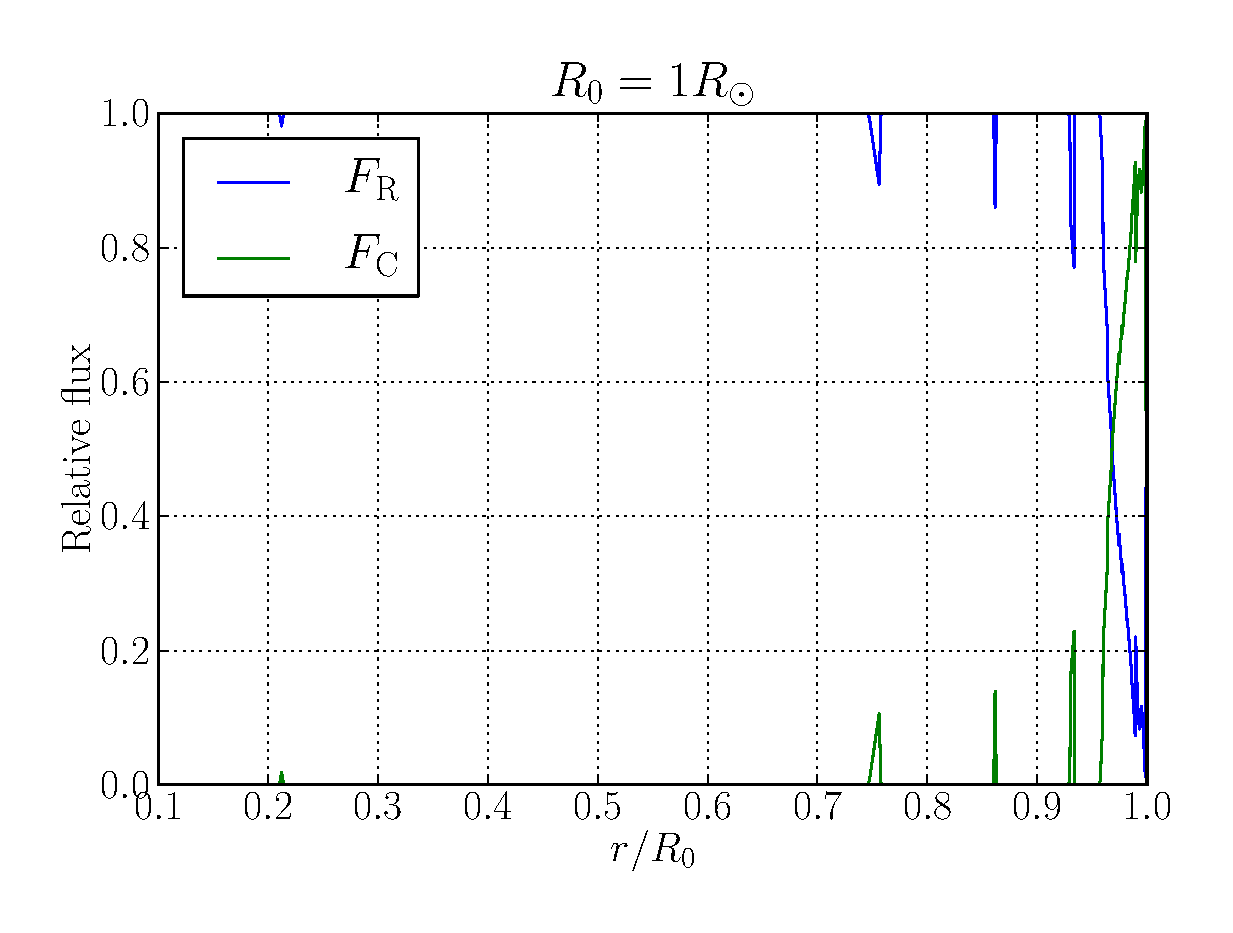
\includegraphics[width=\linewidth]{figures/flux_Rsun.eps}
		\caption{$R = R_{\odot}$}
		\label{fig:flux_Rsun}
	\end{subfigure}\hfill
	\begin{subfigure}{0.49\textwidth}
		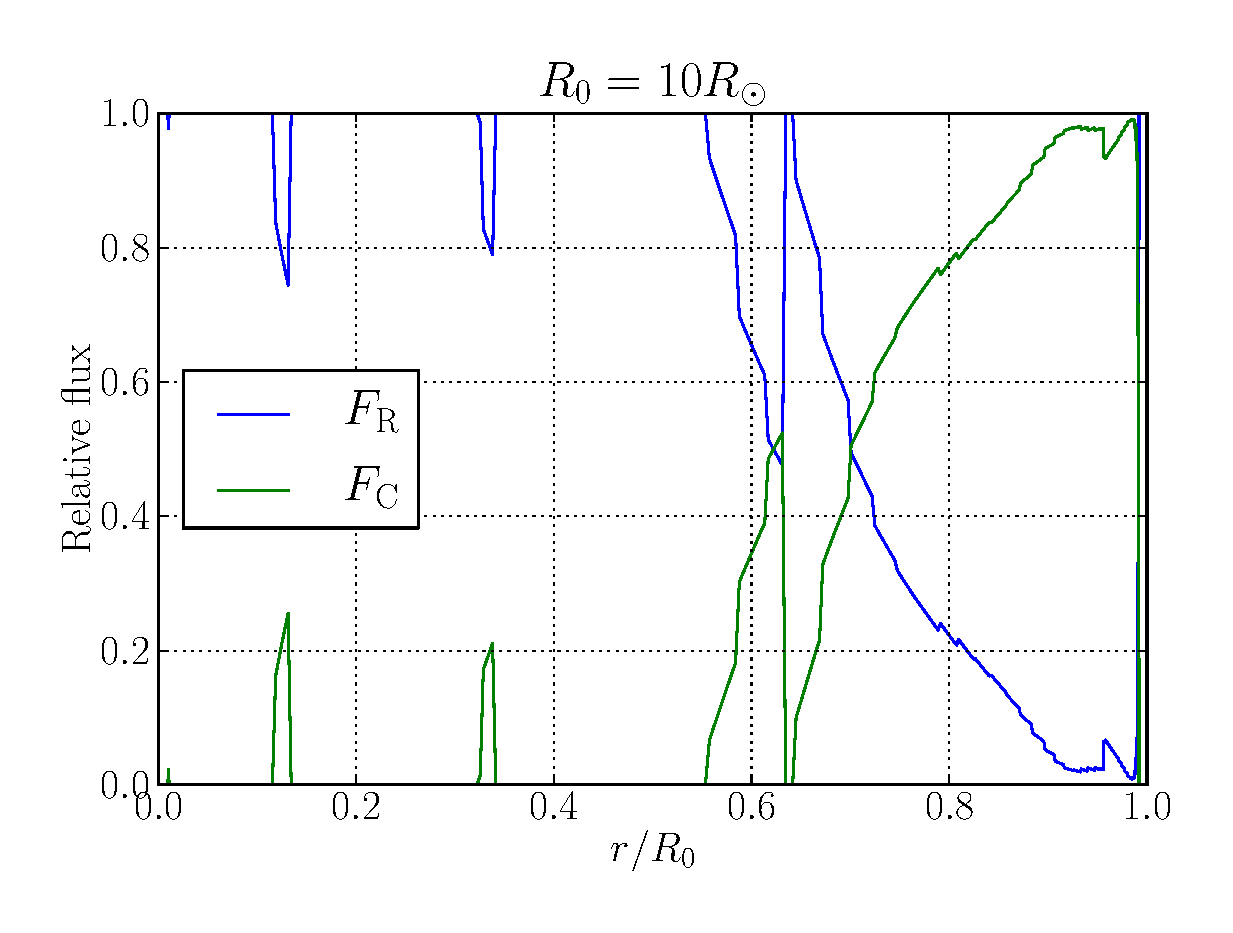
\includegraphics[width=\linewidth]{figures/flux_10Rsun.eps}
		\caption{$R = 10R_{\odot}$}
		\label{fig:flux_10Rsun}
	\end{subfigure}\hfill
	\vspace{0.35cm}
	\begin{subfigure}{0.49\textwidth}
		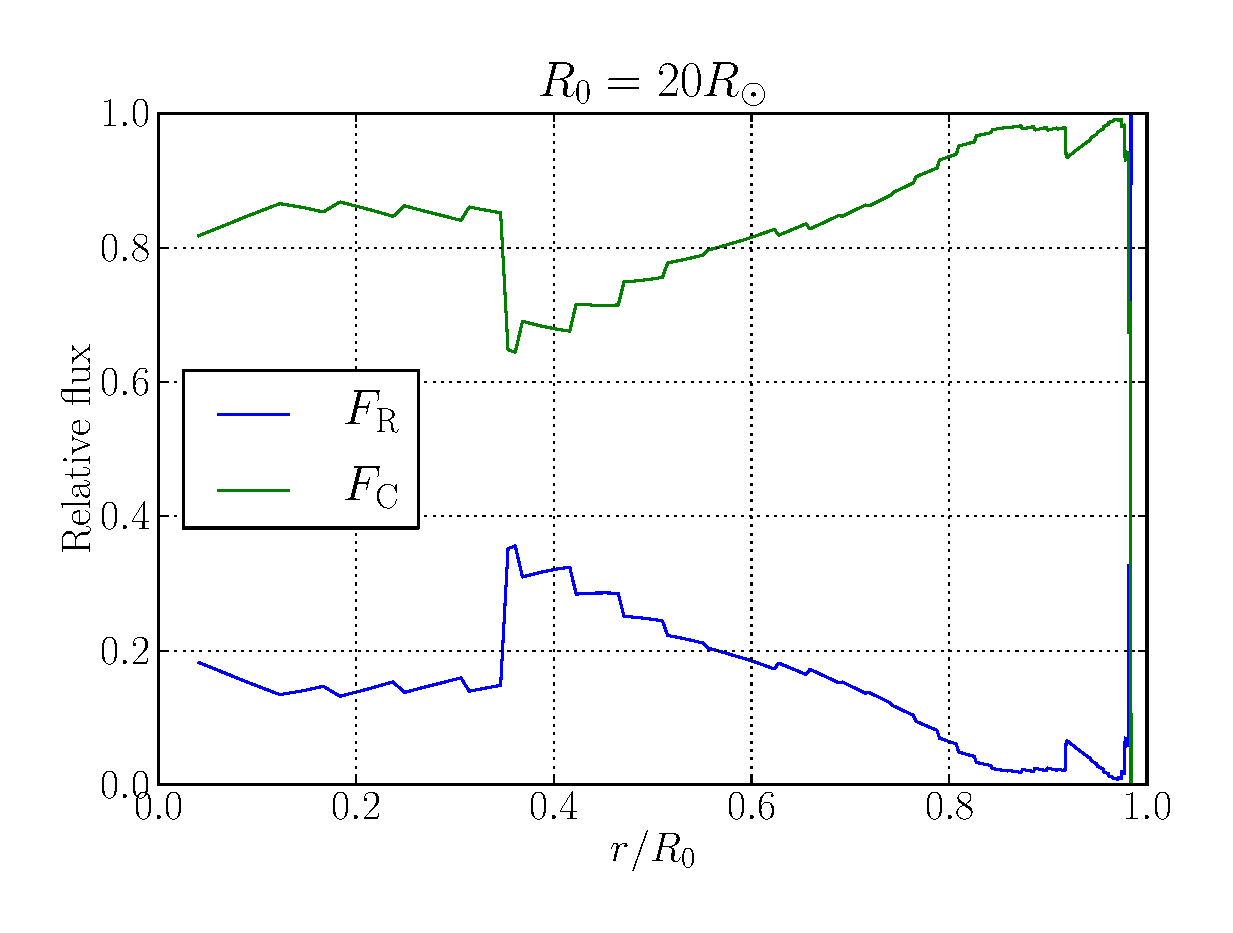
\includegraphics[width=\linewidth]{figures/flux_20Rsun.eps}
		\caption{$R = 20R_{\odot}$}
		\label{fig:flux_20Rsun}
	\end{subfigure}\hfill
	\begin{subfigure}{0.49\textwidth}
		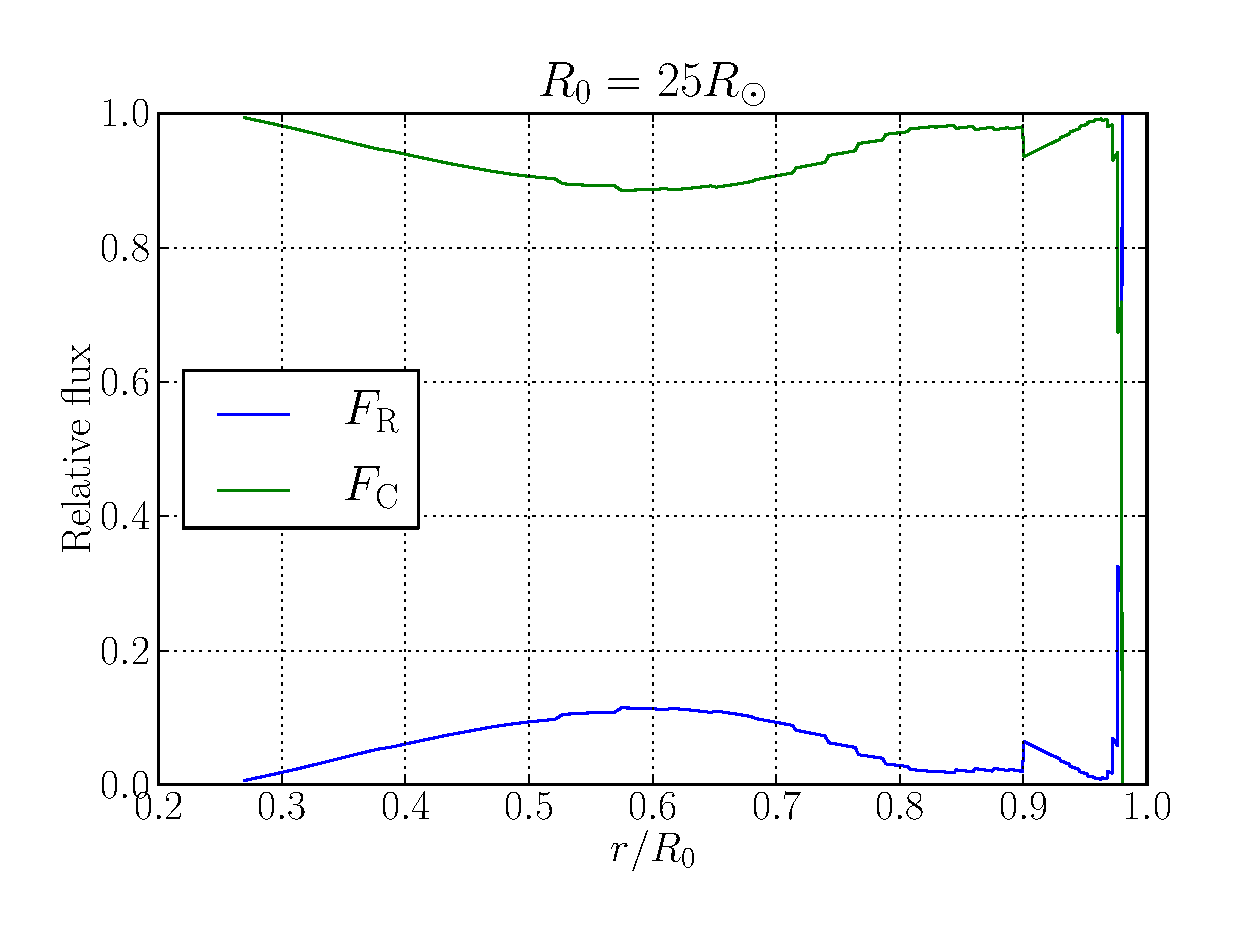
\includegraphics[width=\linewidth]{figures/flux_25Rsun.eps}
		\caption{$R = 25R_{\odot}$}
		\label{fig:flux_25Rsun}
	\end{subfigure}
	\vspace{0.2cm}
	\caption{The change in energy transport for increasing initial stellar radius.}
	\label{fig:flux_change}
\end{figure}

\subsubsection{Energy generation}
We now consider the energy production as function of intitial stellar radius.
Fig.~\refig{energy_Rsun} shows the energy generation for a star like our Sun. We expect
an increase in the energy production towards the core, which we see starts at $R \approx
0.25R_{\odot}$. The PP1-chain is probably what is causing the increase in energy output,
as we see PP2 and PP3 are all very small. An increase in initial radius,
Fig.~\refig{energy_10Rsun}, shows a more sudden and violent jump in energy output. The jump
is much higher in this model, probably because we reach the center of the star, unlike in
the Sun-like case. Increasing the initial radius even more shows a sudden energy
production much earlier. Furthermore, the energy production seems to originate from the
PP3-chain. The energy production is heavily dependent on temperature, so the temperature
must have increased enough for PP3 to be effective.
\begin{figure}[htpb]
	\begin{subfigure}{0.49\textwidth}
		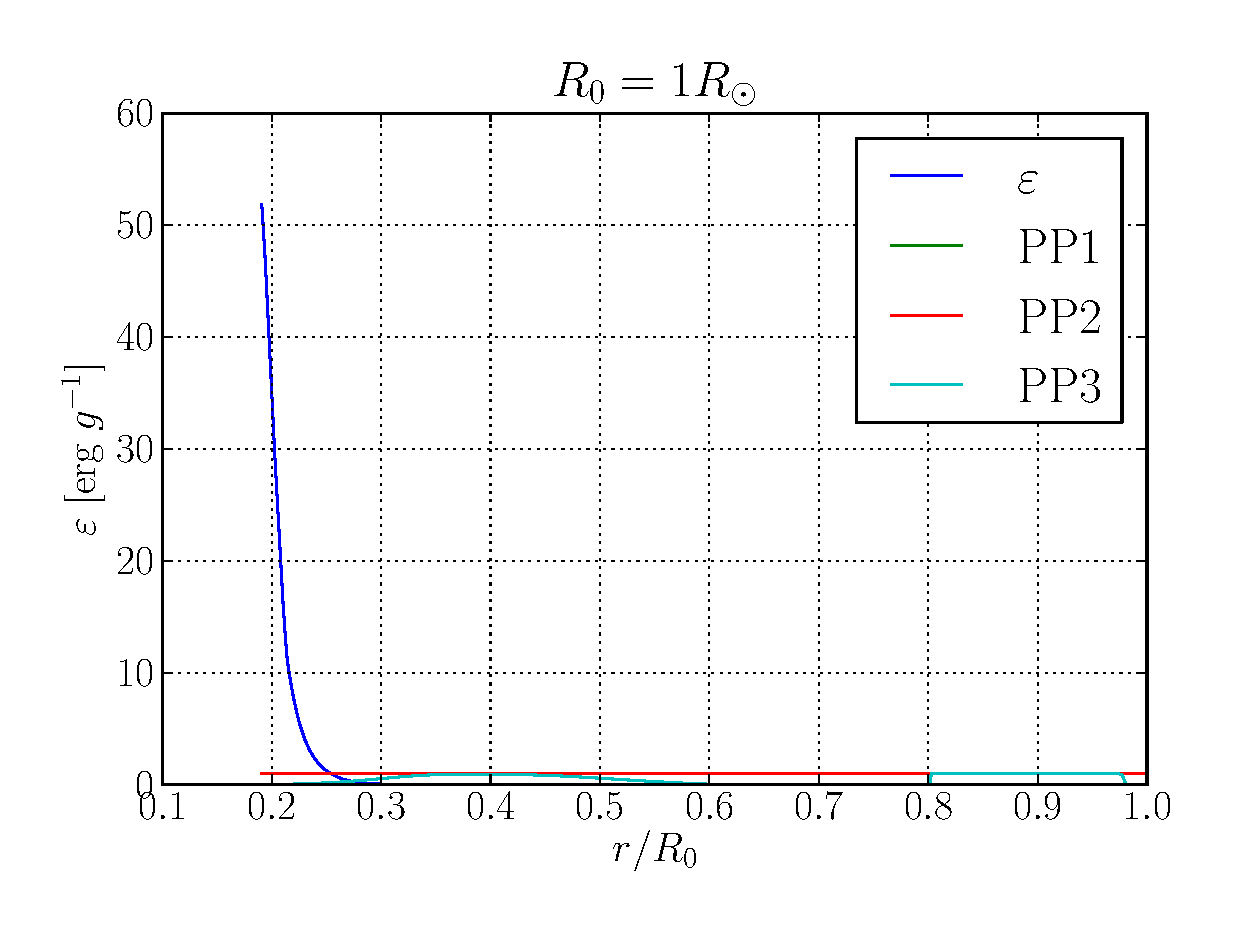
\includegraphics[width=\linewidth]{figures/energy_Rsun.eps}
		\caption{$R = R_{\odot}$}
		\label{fig:energy_Rsun}
	\end{subfigure}\hfill
	\begin{subfigure}{0.49\textwidth}
		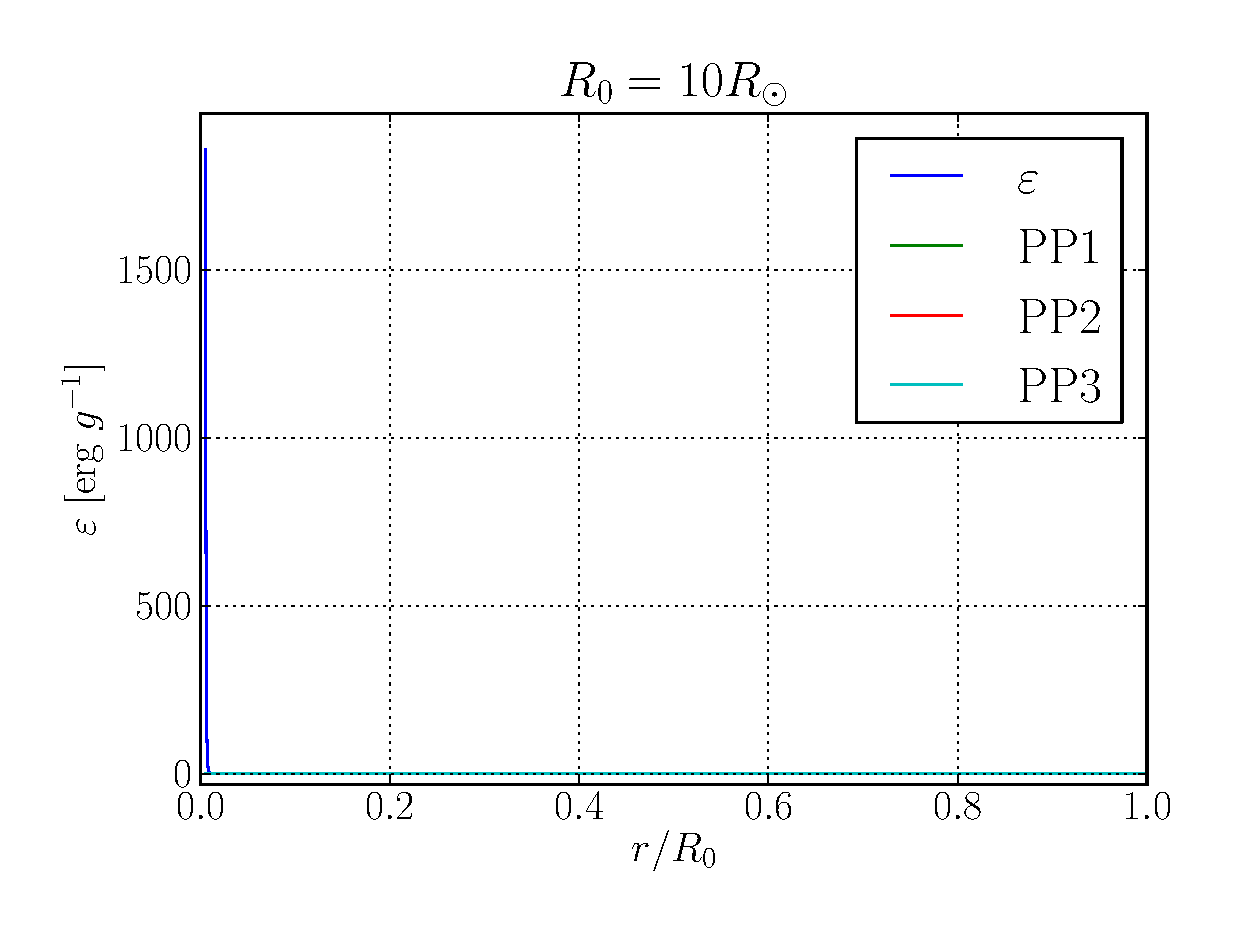
\includegraphics[width=\linewidth]{figures/energy_10Rsun.eps}
		\caption{$R = 10R_{\odot}$}
		\label{fig:energy_10Rsun}
	\end{subfigure}\hfill
	\vspace{0.35cm}
	\begin{subfigure}{0.49\textwidth}
		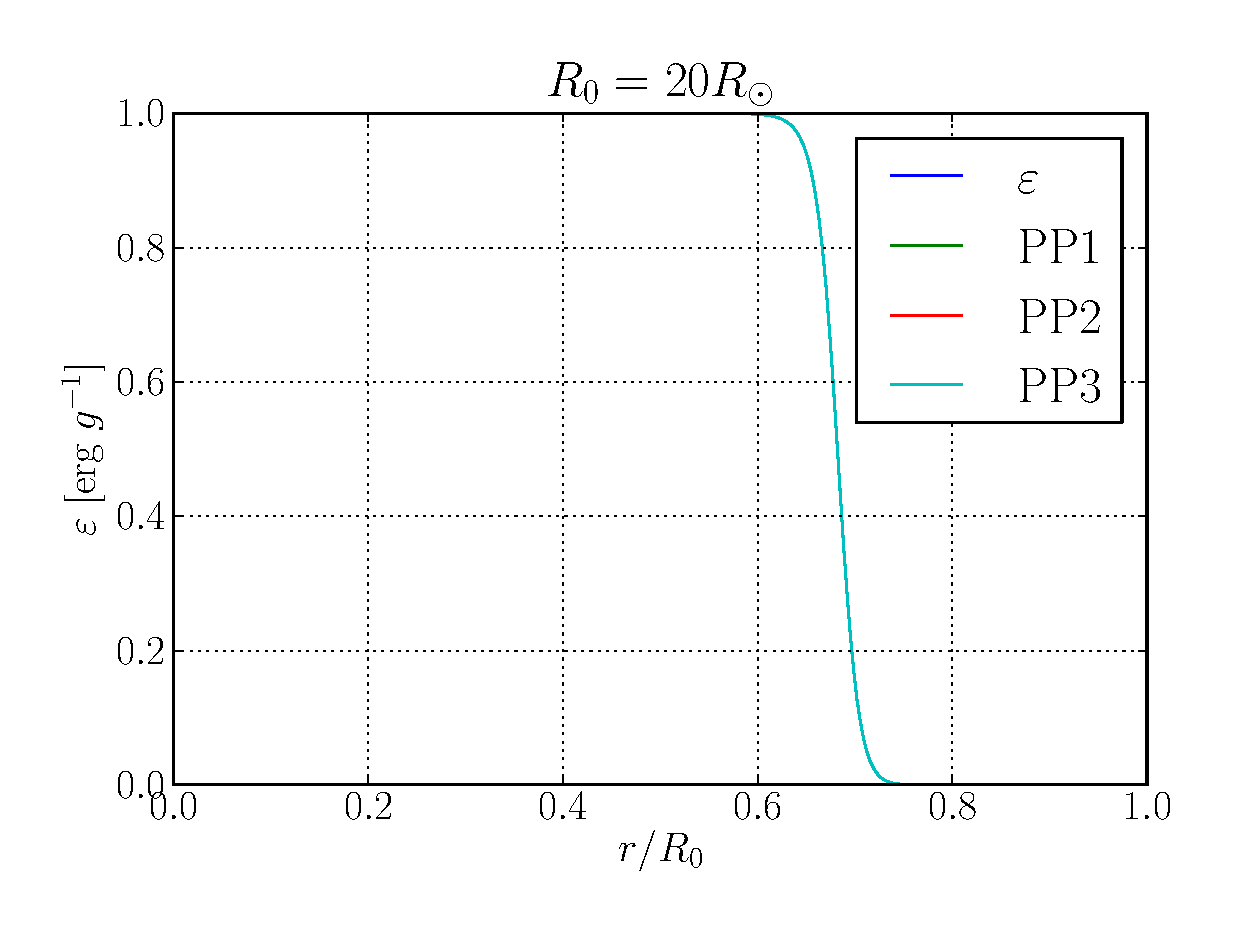
\includegraphics[width=\linewidth]{figures/energy_20Rsun.eps}
		\caption{$R = 20R_{\odot}$}
		\label{fig:energy_20Rsun}
	\end{subfigure}\hfill
	\begin{subfigure}{0.49\textwidth}
		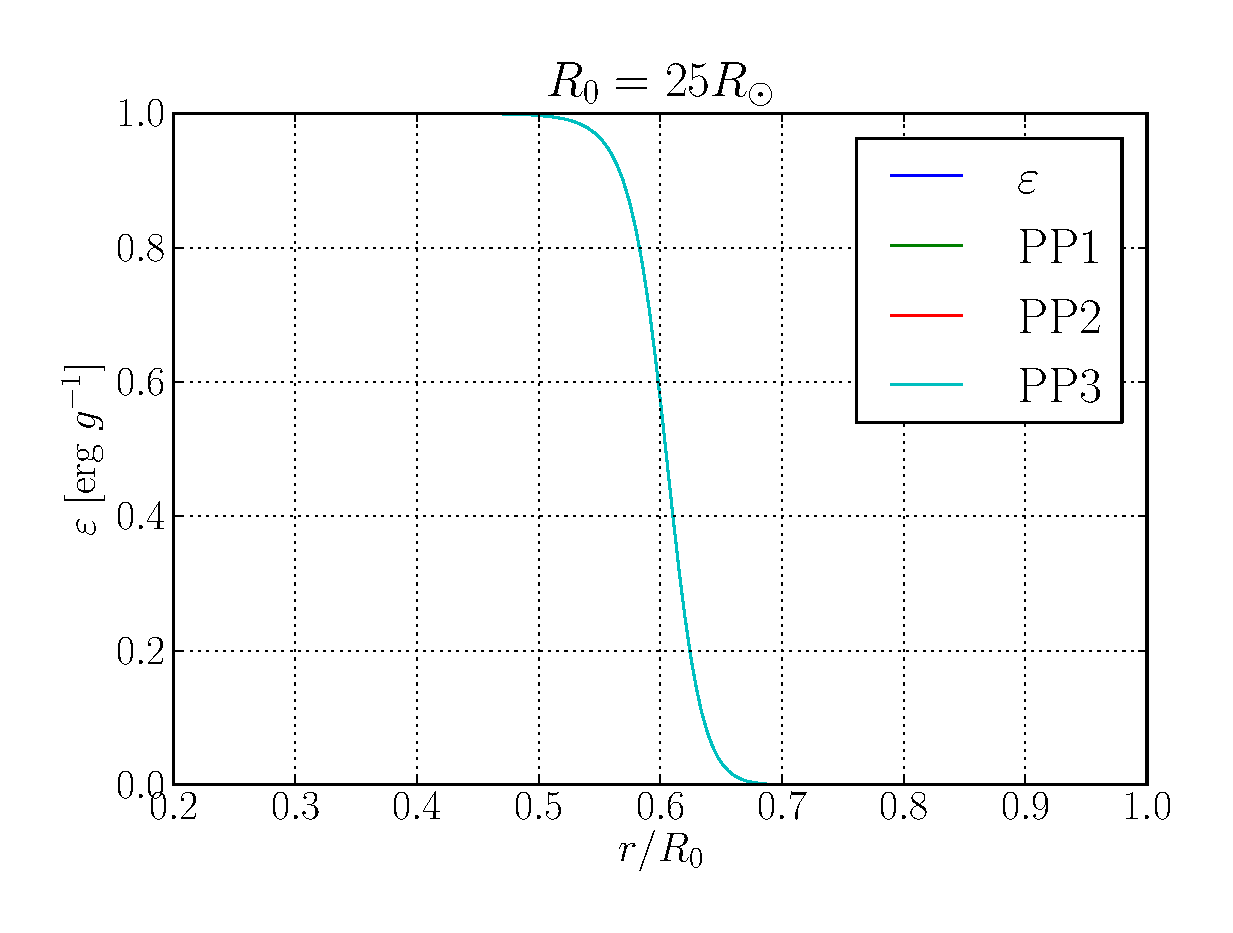
\includegraphics[width=\linewidth]{figures/energy_25Rsun.eps}
		\caption{$R = 25R_{\odot}$}
		\label{fig:energy_25Rsun}
	\end{subfigure}
	\vspace{0.2cm}
	\caption{The change in energy generation for increasing initial stellar radius.}
	\label{fig:energy_change}
\end{figure}

\section{Conclusion}
It is found that the model we implement in this project works better for initial physical
parameters to that of larger and more massive stars than the Sun. We also found the
results to be heavily dependent on how fast the physical parameters change. By applying
constraints to how fast they can change in one step by using an adaptive step method, one
avoids several problems.


\section{The code}
I have provided the link to my GitHub repository below. The code can be found there.

%\lstinputlisting[caption=The program that solves the problem., style=customasm]{../solarCore.py}
\url{}

\begin{thebibliography}{9}
		\bibitem{stix} 
		Michael Stix,
		\emph{The Sun}.
		Springer, New York,
		2nd Edition,
		2002.

		\bibitem{gudiksen}
		Boris Gudiksen
		\emph{AST3310: Astrophysical plasma and stellar interiors}.
		2014.

\end{thebibliography}


\end{document}

